\chapter{Sample}

This is just a sample LaTeX template. \cite{YB}
\section{Basics}

We can simply write $code$ inside plain text. \cite[Kap. 1.2]{Bro11}

We should use footnotes\footnote{this is a footnote} as well.

\subsection{Listings}

\begin{enumerate}
    \item enumerations are fancy
    \item some more..
\end{enumerate}

\begin{itemize}
    \item Just an unordered list
    \item add more..
\end{itemize}

\subsection{Images}

We can reference to images like this: \ref{fig:sample}.

\begin{figure}[h!]
    \centering
    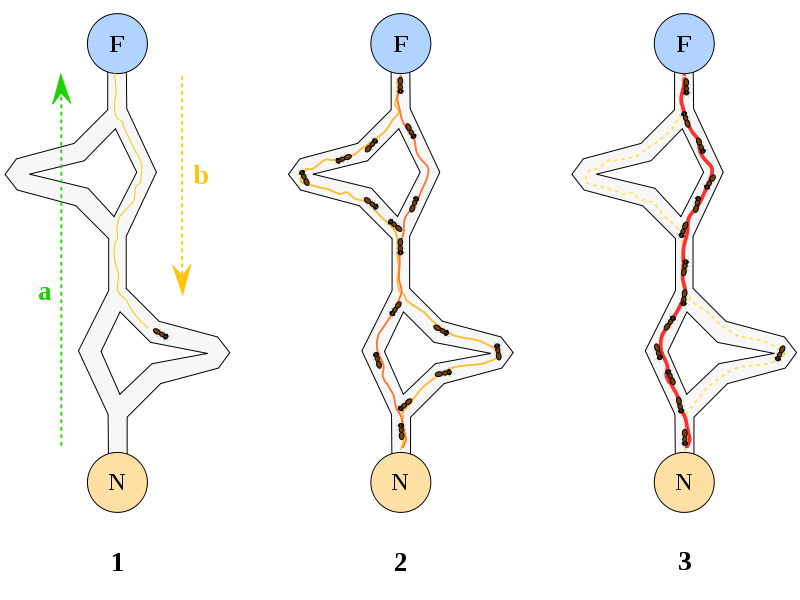
\includegraphics[scale=0.5]{resources/sample.png}
    \caption{this is some sample image \cite{YB}}
    \label{fig:sample}
\end{figure}

\subsection{Maths}

This is some black magic formula:

\begin{equation}
    \label{eq_ant}
    P_{ij}(t) = \begin{cases}
        \frac{[T_{ij}(t)]^\alpha \cdot [N_{ij}]^\beta}
        {\sum_{j \in {allowed}}^{} [T_{ij}(t)]^\alpha \cdot [N_{ij}]^\beta} & \text{wenn } j \in {allowed} \\
        0 & \, \text{sonst}
        \end{cases}
\end{equation}
\label{eq_ant1}

\subsection{Code listings}

We need to define which language to support syntax highlighting.

\begin{lstlisting}[language=Python, caption=Hello World (Python)]
    def hello(name):
        print(f'Hello {name}')
            
\end{lstlisting}

\subsection{Tables}

% \addcontentsline{lot}{table}{This adds the table to the list of tables}
\begin{tabular}{l*{6}{c}r}
    Team              & P & W & D & L & F  & A & Pts \\
    \hline
    Manchester United & 6 & 4 & 0 & 2 & 10 & 5 & 12  \\
    Celtic            & 6 & 3 & 0 & 3 &  8 & 9 &  9  \\
    Benfica           & 6 & 2 & 1 & 3 &  7 & 8 &  7  \\
    FC Copenhagen     & 6 & 2 & 1 & 3 &  5 & 8 &  7  \\
\end{tabular}
\captionof{table}{Champions League Group D}\label{tbl:football}